\documentclass{crypto-exercise}
\author{Sven Laur}
\contributor{Karl Tarbe}
\editor[Added illustrations]{Sven Laur}
\tags{Merkle tree, collision resistance, binding}

\newcommand{\GETROOT}{\mathsf{GetRoot}}

\begin{document}
\begin{exercise}{Merkle trees are binding commitments}
Show that Merkle tree is a binding commitment if the underlying hash function family $\HHH$ is $(t,\varepsilon)$-collision resistant. Recall that Merkle tree is a binary tree with vertices $(c_{ij})$, where intermediate leafs are computes as
\begin{align*}
c_{ij}=h(c_{i+1,2j},c_{i+1,2j+1}), \qquad i\in\set{0,\ldots, k-1},\quad j\in\set{0,\ldots 2^i-1}
\end{align*} 
and leafs $c_{k,j}$ for $j\in\set{0,2^k-1}$ are messages to be committed. The commitment digest is $c_{00}$ and to open a message $c_{k,j}$ you have to open minimal number of leaks and intermediate vertices needed to compute $c_{00}$. A commitment is valid, if one indeed obtains $c_{00}$ from the released messages.  
\end{exercise}

\begin{solution}
Let us first illustrate how one uses Merkle tree to commit a bitstring $m$ consisting of eight blocks $m_7,\ldots, m_0\in\MSPACE$. Note that the hash function $h$ used to compute the commitment digest $c_{00}$ must be of type $h:\MSPACE\times\MSPACE\to\MSPACE$. In order to commit the message $m$, we first treat its blocks as third level nodes in the Merkle tree and compute the values of intermediate nodes $c_{ij}$ according to the specification. Let $\GETROOT$ be the corresponding algorithm that computes the root of the hash tree, as illustrated below.
\begin{center}
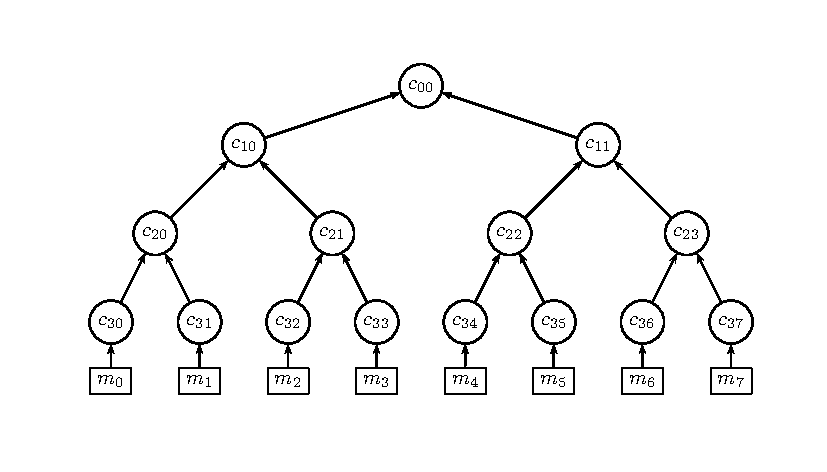
\includegraphics[trim=0cm 1cm 0cm 1cm, clip]{./figures/0701-merkle-tree}
\end{center}
In order to double open the commitment $c_{00}$, one must produce alternative message $\overline{m}$ consisting also from eight blocks $\overline{m}_7,\ldots, \overline{m}_0$ such that the digest computation leads to the same result. More generally, we are interested what is the best advantage against the binding game: 
\begin{align*}
    \begin{game}{\GAME}
      & h \gets \HHH\\
      & (c_{00},m,\overline{m}) \gets \AD(h)\\
      & \IF c_{00}\neq\GETROOT(m)\ \THEN \RETURN 0\\
      & \IF c_{00}\neq\GETROOT(\overline{m})\ \THEN \RETURN 0\\
      & \RETURN [m \neq \overline{m}]
    \end{game}
\end{align*}
where the third and fourth line check that the $c_{00}$ is indeed a valid commitment to $m$ and $\overline{m}$. Also, note that the public parameter of the commitment scheme is the description of a hash function $h$ and public parameter generation is random sampling of an hash function. 

It is straightforward to see that Merkle tree without additional restrictions is not binding at all. For example, let $c_{00}$ be the digest corresponding to the message blocks $m_0,\ldots, m_7$. Then four block message $\overline{m}$ consisting intermediate values:
\begin{align*}
 c_{20}=h(m_0,m_1),\quad
 c_{21}=h(m_2,m_3),\quad
 c_{22}=h(m_4,m_5),\quad
 c_{23}=h(m_6,m_7)
\end{align*}
leads to the same digest $c_{00}$. Hence, we must clarify the definition of the Merkle tree commitments by requiring that the number of layers $k$ is fixed, as implicitly suggested by the exercise text. 

Next, we prove that  commitment scheme based on the Merkle tree with $k$ levels is a binding under the assumption that the hash function family $\HHH$ is $(t,\varepsilon)$-collision resistant. For that, we must convert an adversary $\AD$ against the binding game $\GAME$ to another adversary $\ADB$ that can break collision resistance property
of the underlaying hash function family $\HHH$. Recall that the collision resistance property of an hash function family is defined through the following game:
\begin{align*}
    \begin{game}{\BGAME}
      & h \getsu \HHH \\
      & (x_0,x_1) \gets \ADB(h) \\
      & \IF x_0 = x_1\ \THEN \RETURN 0\\
      & \RETURN [ h(x_0) \iseq h(x_1)] \enspace.
    \end{game}
\end{align*}
Assume that $\AD$ returns a valid double opening $(c_{00}, m, \overline{m})$. Then there must be two instances of Merkle trees with the same root node that can be aligned, as illustrated below. 

\begin{center}
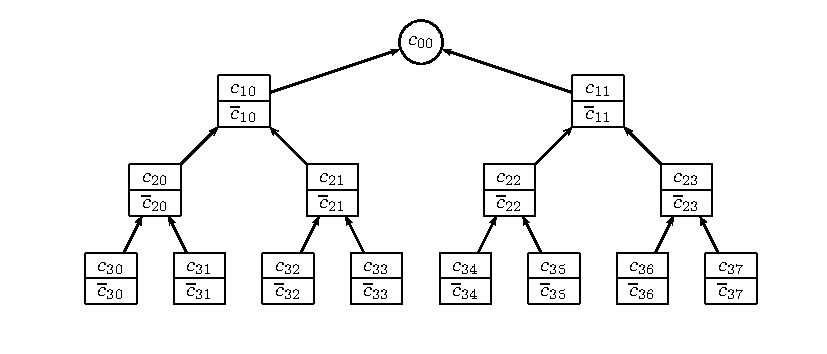
\includegraphics[trim=0cm 0.5cm 0cm 0cm, clip]{./figures/0701-double-opening}
\end{center}

More formally, let $c_{ij}$ denote the intermediate values corresponding to the message $m$ and let $\overline{c}_{ij}$ denote intermediate values corresponding to the message $\overline{m}$. It is easy to see that if the root of a subtree $c_{i,j}$ has the same value has $\overline{c}_{i,j}$, then we have either identical children: $c_{i+1,2j}=\overline{c}_{i+1,2j}$ and $c_{i+1,2j+1}=\overline{c}_{i+1,2j+1}$ or there is an explicit hash collision:
\begin{align*}
(c_{i+1,2j}, c_{i+1,2j+1})&\neq (\overline{c}_{i+1,2j}, \overline{c}_{i+1,2j+1})\enspace,\\
h(c_{i+1,2j}, c_{i+1,2j+1})&=h(\overline{c}_{i+1,2j}, \overline{c}_{i+1,2j+1})\enspace.
\end{align*}
By applying this observation recursively, we either discover a hash collision or all vertices in the tree are identical. The latter cannot happen as $m\neq\overline{m}$ in case of valid double opening.

Hence, we can extract hash collision from a double opening by splitting the messages $m$ and $\overline{m}$ into the $k$th layer values $c_{k,j}$ and $\overline{c}_{k,j}$ and then computing the values $c_{ij}$ and $\overline{c}_{ij}$ of next layers until we find the hash collision. The corresponding adversary is depicted below:
\begin{align*}
    \begin{game}{\ADB(h)}
        & (c_{00},m,\overline{m}) \gets \AD(h)\\
        & \text{Let $c_{k0},\ldots, c_{k2^k-1}$ be the block representation of $m$.}\\
        & \text{Let $\overline{c}_{k0},\ldots, \overline{c}_{k2^k-1}$ be the block representation of $\overline{m}$.}\\
        & \begin{forblock}{i \in (k,\ldots,1)\ }
           &\begin{forblock}{j\in (0,\ldots 2^{k-1}-1)\ }
            & x_0\gets (c_{i,2j}, c_{i,2j+1})\\
            & x_1\gets (\overline{c}_{i,2j}, \overline{c}_{i,2j+1})\\
            & c_{i,j} \gets h(c_{i,2j}, c_{i,2j+1})\\
            & \overline{c}_{i,j} \gets h(c_{i,2j}, c_{i,2j+1})\\
            & \hat{c}_{i-1,j} \gets h(\overline{c}_{i,2j}, \overline{c}_{i,2j+1})\\
            &\begin{ifblock}{c_{i,j} = \overline{c}_{i,j}\wedge x_0\neq x_1\ }
              & \RETURN (x_0, x_1)
            &\end{ifblock}
           \end{forblock}
        \end{forblock}\\
        & \RETURN \bot
    \end{game}
\end{align*}
Note that $\ADB$ is guaranteed to succeed if $\AD$ provides a valid double opening, since the condition inside the second loop must be met for some iteration by the reasoning given above. Hence, we have established 
\begin{align*}
\pr{\BGAME^\ADB = 1}\geq\pr{\GAME^\AD = 1}\enspace.
\end{align*}
Note that $\ADB$ can be more successful than $\AD$, as invalid double opening might still reveal the hash collision. Of course, the probability of such events is negligible for reasonable adversaries.   

Note that the running-time of $\ADB$ is $t_\AD + \Theta(2^k)$, where $t_\AD$ is the running-time of $\AD$ and $k$ is the height of the tree. At first glance the overhead $\Theta(2^k)$ seems worrisome, as it seems to lead to exponential slowdown. However, note that $k$ must be small in practical applications as the length of the committed message is also $\Theta(2^k)$ and the time needed to verify the digest is also $\Theta(2^k)$. In fact, the overhead of $\ADB$ roughly corresponds to the verification of both decommitments.  As a result, we still obtain a tight connection between the collision resistance and binding property. Namely, if the hash function family $\HHH$ is $(t,\varepsilon)$-collision resistant, then Merkle tree commitment is $(t-\Theta(2^k),\varepsilon)$-binding.

\end{solution}



\end{document}
